\documentclass{article}


% if you need to pass options to natbib, use, e.g.:
%     \PassOptionsToPackage{numbers, compress}{natbib}
% before loading neurips_2023


% ready for submission
\usepackage[final]{neurips_2023}


% to compile a preprint version, e.g., for submission to arXiv, add add the
% [preprint] option:
%     \usepackage[preprint]{neurips_2023}


% to compile a camera-ready version, add the [final] option, e.g.:
%     \usepackage[final]{neurips_2023}


% to avoid loading the natbib package, add option nonatbib:
%    \usepackage[nonatbib]{neurips_2023}


\usepackage[utf8]{inputenc} % allow utf-8 input
\usepackage[T1]{fontenc}    % use 8-bit T1 fonts
\usepackage{hyperref}       % hyperlinks
\usepackage{url}            % simple URL typesetting
\usepackage{booktabs}       % professional-quality tables
\usepackage{amsfonts}       % blackboard math symbols
\usepackage{nicefrac}       % compact symbols for 1/2, etc.
\usepackage{microtype}      % microtypography
\usepackage{xcolor}         % colors

\usepackage[pdftex]{graphicx}
\graphicspath{{./graphs/}}

\title{Procesamiento de imágenes (pre TP1)}

\author{
  Víctor A.~Bettachini\\ %\thanks{Use footnote for providing further information about author (webpage, alternative address)---\emph{not} for acknowledging funding agencies.} \\
  Datamining en ciencia y tecnología 2023\\
  Especialización en Explotación de Datos y Descubrimiento del Conocimiento\\
  \texttt{bettachini@gmail.com}
}


\begin{document}


\maketitle


\begin{abstract}
Cuca.
\end{abstract}


\section{Introducción}

\section{Materiales y métodos}

\paragraph{Datos}
210 imágenes de flores acompañados de un listado de las correspondientes especies dentro de una variedad de 10.
Las imágenes en formato png tienen una dimensión de 128 x 128 píxeles con tres canales de color.
El conjunto se descargó de una fuente pública [2].

\paragraph{Recurso informático} 
Un cuaderno (notebook) Jupyter provisto por los docentes en el sitio web denominado ``Campus'' [1] provee un marco donde escribir el código en lenguaje Python que explote la biblioteca Clustimage para el trabajo con imágenes.
El mismo se publica como un enlace para ejecutarle en el servicio en línea Google Colaboratory.
Se modificó el sendero a los archivos para indicar un directorio en un sistema de archivos local de una computadora local para ejecutarle con mayor velocidad.


\section{Resultados}
% \section{Lo realizado}
Cada actividad realizada se describe bajo los titulos que figuran en el enunciado del trabajo práctico publicado en el


Análisis de componentes principales
Una centena de componentes principales por imagen se obtuvieron con el método \verb'exctract_feat' [3].



\section{Discusión}

\begin{figure}
  \centering
  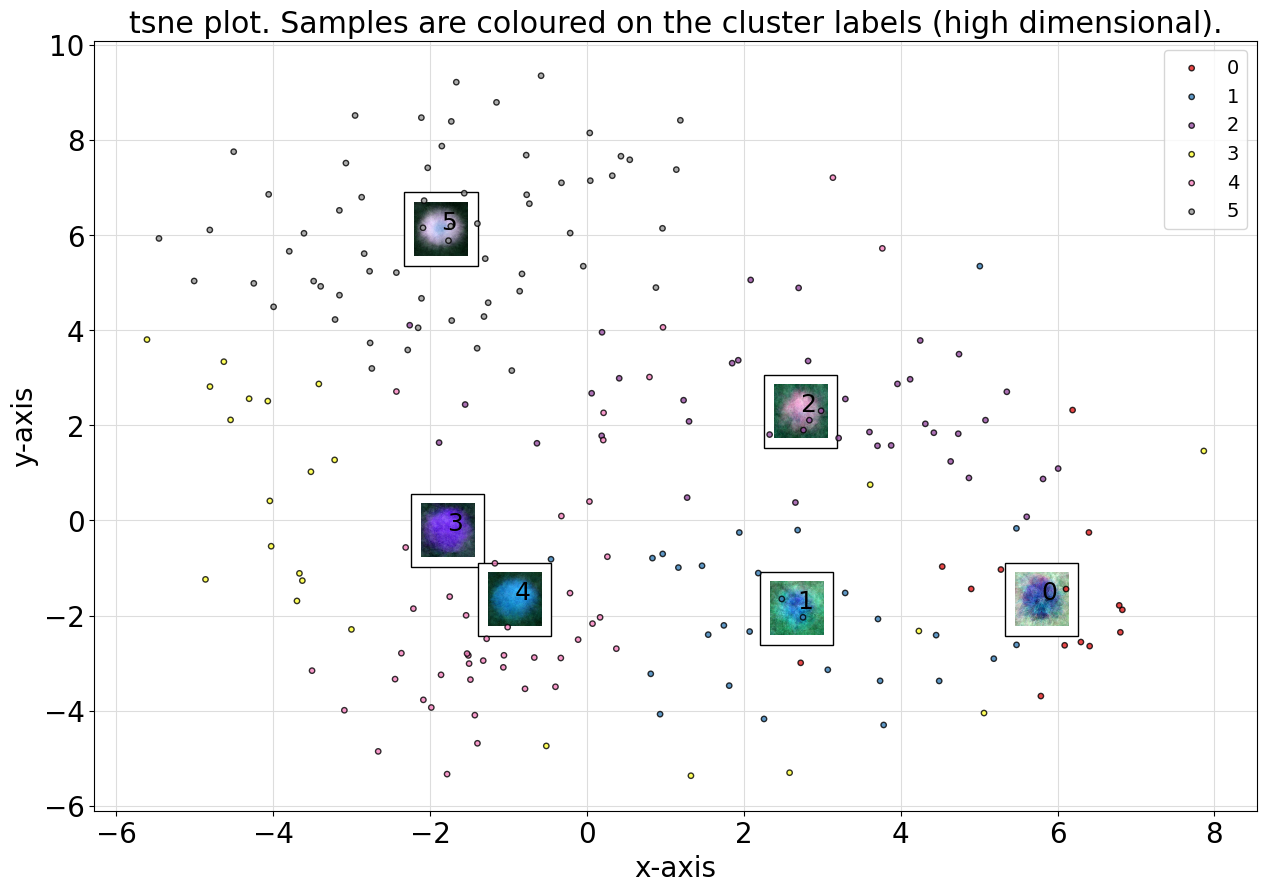
\includegraphics[width= 0.8\linewidth]{tsne}
  \caption{Ubicación de cada imágen en componentes principales(tsne plot)}
\end{figure}

\section*{References}

\medskip
{
\small

[1] Kamienkowski, J.A.\ \& \emph{et al.} (2023) {\it Campus de Datamining en ciencia y tecnología}, \url{https://datamining.dc.uba.ar/campus/course/view.php?id=37}

[2] Olga Belitskaya (2020, última actualización) Flower Color Images, {\it Kaggle}, \url{https://www.kaggle.com/olgabelitskaya/flower-color-images}

[3] Taskesen, E. (2020) PCA, {\it clustimage's documentation!}, \url{https://erdogant.github.io/clustimage/pages/html/Feature%20Extraction.html}
}

%%%%%%%%%%%%%%%%%%%%%%%%%%%%%%%%%%%%%%%%%%%%%%%%%%%%%%%%%%%%


\end{document}